\documentclass[10pt]{standalone}
\usepackage{tikz}
\usepackage{lmodern}
\usepackage[T1]{fontenc}
\usepackage[utf8]{inputenc}
\usepackage{amsmath}
\usepackage{mathtools}
\usepackage{graphicx}
\usepackage{bbm}
\usepackage[margin=1in]{geometry}
\usepackage{caption}
\usepackage{subcaption}
\usepackage{float}
\usepackage{tikz}

\usepackage[RPvoltages]{circuitikz}

\usetikzlibrary{decorations.pathreplacing,angles,quotes}

\usepackage{tikz,bm} % Useful for drawing plots
%\usepackage{tikz-3dplot}
\usetikzlibrary{shapes.geometric, arrows}
\tikzstyle{process} = [rectangle, rounded corners, minimum width=2cm, minimum height=0.8cm, text centered, draw=black, fill={rgb, 255:red, 150; green, 150; blue, 150 }, line width=0.5mm]
\tikzstyle{processr} = [rectangle, rounded corners, minimum width=2cm, minimum height=0.8cm, text centered, draw=black, fill={rgb, 255:red, 211.65; green, 175.95; blue, 56.1 }, line width=0.5mm]

\tikzstyle{decision} = [rectangle, rounded corners, minimum width=2.5cm, minimum height=1cm, text centered, draw=black,fill= {rgb, 255:red, 136; green, 182; blue, 168 } , line width=0.5mm]
\tikzstyle{legend} = [rectangle, minimum width=5cm, minimum height=2cm, , draw=black,fill=white, line width=1mm]
\tikzstyle{legend2} = [rectangle, minimum width=5cm, minimum height=3cm, , draw=black,fill=white, line width=1mm]
\tikzstyle{arrow} = [thick,->,>=stealth]
\usetikzlibrary{positioning}
\usetikzlibrary{calc}
\usepackage{circuitikz}


\usepackage{genealogytree}
\gtruselibrary{templates}
\usetikzlibrary{arrows.meta,positioning}
\usepackage[figurename=Figure]{caption} %
\usepackage{amsfonts} %
\usepackage{xcolor} %
\usepackage{enumitem}
\title{Extract from Notes}
\author{Zak Gittins, Alexander Kaye, Byron Tzamarias}
\date{}
\begin{document}
	
	\begin{minipage}{\linewidth}
		\centering
		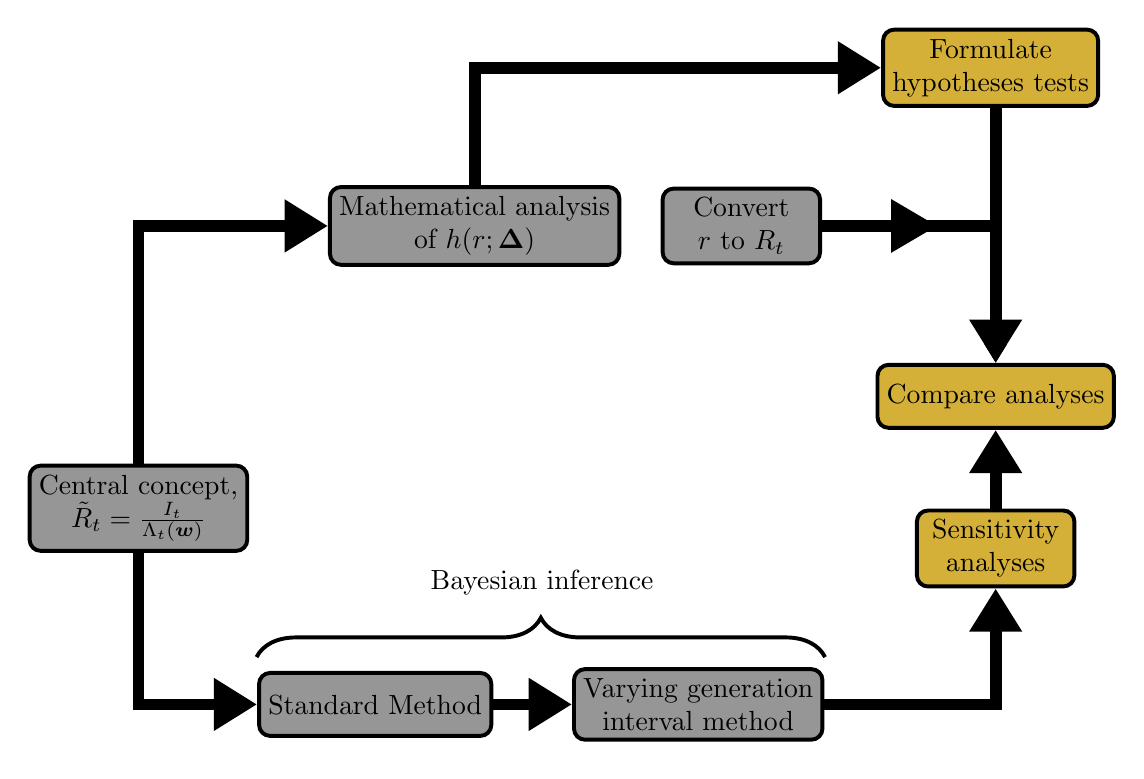
\begin{tikzpicture}[node distance=2cm, every text node part/.style={align=center}]
		
		\node (main_concept) [process] {Central concept,\\$\tilde{R}_t = \frac{I_t}{\Lambda_t(\boldsymbol{w})}$};
		
		\node (standard_method) [process,below right = 1.5cm and .1cm of  main_concept] {Standard Method};
		\node (math) [process,above right = 2.5cm and 1cm of  main_concept] {Mathematical analysis\\of $h(r;\boldsymbol{\Delta})$};
		
		\node (alter_method) [process,right = 1cm of  standard_method] {Varying generation\\interval method};
		\node (sensitivity) [processr,above right =  1cm and 1.15cm of  alter_method] {Sensitivity\\analyses};
		\node (r_to_R) [process,right = .5cm of math] {Convert\\$r$ to $R_t$};
		\node (hyp_test) [processr,above right = 1cm and 0.75cm of  r_to_R] {Formulate\\hypotheses tests};
		
		% \node (time) [below right= 3.5cm and 3.5cm of main_concept] {\textbf{Time}};
		
		\node (compare) [processr, above = 1cm of sensitivity] {Compare analyses};
		
		\node (meeting) [above = 2cm of compare]{};
		
		
		
		% \draw [-{Triangle[scale=1.0]}, line width = 1.5mm, color=black!60!blue] ([yshift = -4.2cm] main_concept.south) --   ([yshift = -4.2cm, xshift = 10cm]main_concept.south);
		
		% \draw [-{Triangle[scale=1.0]}, line width = 1.5mm, opacity=0] ([xshift = -2cm, yshift = -4.4cm] main_concept.south) --   ([yshift = -4.2cm, xshift=-0.1cm]main_concept.south);
		
		\draw [-{Triangle[scale=1.0]}, line width = 1.5mm] (main_concept.north) |- node[above right]{} (math.west);
		\draw [-{Triangle[scale=1.0]}, line width = 1.5mm] (main_concept.south) |- node[above right = 1.2cm and 3.52cm ]{Bayesian inference} (standard_method.west);
		
		\draw [-{Triangle[scale=1.0]}, line width = 1.5mm ] (standard_method.east) --  (alter_method.west);
		\draw [-{Triangle[scale=1.0]}, line width = 1.5mm ] (alter_method.east) -| (sensitivity.south);
		
		%\draw [ -{Triangle[scale=1.0]}, line width = 1.5mm] (NL.east) -- +(1,0)|- node[above right]{} (NLN.west);
		%\draw [-{Triangle[scale=1.0]}, line width = 1.5mm] (NL.east) -- +(1,0)|- node[above right]{} (NLL.west);
		
		
		% \draw [-{Triangle[scale=1.0]}, line width = 1.5mm ] (math.south) |- (compare);
		
		\draw [-, line width = 1.5mm ] (r_to_R.east) -- ([xshift = 2.2cm, yshift = 0cm] r_to_R.east) node[
		currarrow,
		pos=0.5,
		xscale = 0.8,
		scale=3]{};
		
		\draw [-{Triangle[scale=1.0]}, line width = 1.5mm] ( math.north) |- (hyp_test.west);
		
		\draw [-{Triangle[scale=1.0]}, line width = 1.5mm ] ([xshift = 0cm, yshift = 4.11cm] compare.south) -- (compare.north);
		
		\draw [-{Triangle[scale=1.0]}, line width = 0.5mm ] ([xshift = 0cm, yshift = 3.75cm] compare.south) -- (compare.north);
		
		\draw [-{Triangle[scale=1.0]}, line width = 1.5mm ] (sensitivity.north) -- (compare.south);
		
		% \draw [dashed, line width=.5mm] (8.86,-5) -- (8.86,6);
		
		% \draw[line width = 0.5mm, decoration={brace,mirror,raise=5pt, amplitude = 0.2cm },decorate]([xshift = -1cm, yshift = -3cm] main_concept.south) -- node[below=0.75cm] {Methods} ([xshift = 9.5cm, yshift = -3cm] main_concept.south)
		\draw[line width = 0.5mm, decoration={brace,mirror,raise=5pt, amplitude=0.5cm },decorate, rotate=0]([xshift = 8.72cm, yshift = -1.5cm] main_concept.south) -- node[below=0.75cm] {} ([xshift = 1.5cm, yshift = -1.5cm] main_concept.south);
		
		
		% \filldraw [-{Triangle[scale=1.0]}, line width = 1.5mm, color = gray] ([xshift = -2cm, yshift = -1cm] Default.south) --   ([yshift = -1cm, xshift = -1cm]Default.south);
		% \draw [-{Triangle[scale=1.0]}, line width = 1.5mm] ([yshift = -2cm, xshift = -2cm] Default.south) --   ([yshift = -2cm, xshift = -1cm]Default.south);
		% \draw [dashed, -{Triangle[scale=1.0]}, line width = 1.5mm ] ([xshift = -2cm, yshift = -3cm] Default.south) --   ([yshift = -3cm, xshift = -1cm]Default.south);
		
		% \node (lg1) [below right = 0.75cm and -2cm  of Default] {High uncertainty};
		% \node (lg2) [below right = 1.75cm and -2cm  of Default] {Low uncertainty};
		% \node (lg3) [below right = 2.75cm and -2cm  of Default] {Monitoring};
		
		
		% \node (t_1) [legend, above = 0.5cm of Default] {};
		
		
		% \node (lgb) [above left = 0.75cm and -0.1cm  of Default] {$\boldsymbol{L}$:};
		% \node (lgc) [above left = 1.75cm and -0.1cm  of Default] {$\boldsymbol{N}$:};
		
		
		% \node (lgB) [above right = 0.75cm and -2cm  of Default] {Lockdown};
		% \node (lgC) [above right = 1.75cm and -2cm  of Default] {No lockdown};
		
		
		
		\end{tikzpicture}
		
		\label{fig:rates}
	\end{minipage}
	
\end{document}

\\
